% Postface

%\newgeometry{marginparwidth=2.5cm, marginparsep=2cm} 

\chapter{Postface}
\fancyhead[LO]{Postafce}

\lettrine[lines=3]{J}{e dois avouer} que l’écriture de cette pièce, pourtant fort courte au regard des autres ouvrages que j’ai donné par le passé, m’a été une tache exténuante. C’est que le sujet et l’atmosphère de cette pièce, s’ils sont particulièrement violents pour les personnages le furent aussi pour l’auteur. Car il m’a semblé que l’écriture, si elle est bien menée, n’est pas un acte désincarné ; aussi, à chaque fois que je saisissais le clavier pour en écrire les répliques, je croyais toucher de mes doigts les touches et c’est sur la barre de l’Arche que mes mains se posaient. Une barre brulante, parsemée de pics et de bris de verre. J’étais alors propulsé à la cour de \campprincipal, au milieu des ambitieux intrigants aux canines si longues qu’elles lacèrent le parquet, au milieu du sang qui dispute son débit aux larmes, au milieu de la chaire humaine qui se broie industriellement. S’il est des murs qui ont des oreilles, ceux de l’Arche ont des bras et des mains tenant les poignards prompts à transpercer les benêts qui croiraient pouvoir s’y adosser sereinement. Ce n’est pas que dans le replis des toges que se drapent les lames assassines mais aussi dans le marbre et la maçonnerie pourtant lisses et rigides. C’est un univers sans répit où chaque aspiration se paie et chaque expiration se rembourse.

Il n’est pas anodin à cet égard de constater que la musique qui m’accompagna lors de cette rédaction est celle du studio audiomachine, dont le style calibré pour la musique de cinéma est épique. Et plus particulièrement leur album \work{Greatest Hits}\footnote{\textsc{audiomachine} : \work{Greatest Hits}. 2022.} dans lequel je trouvais des accents encore plus violents que les précèdent et qui à cet égard me semblèrent propice à être insufflés à la diégèse de cette œuvre.

\paragraph{Graphomachie}
Une violence, dis-je, et même une douleur qui surgissent de la typographie du texte pour m’asséner des coups à la mâchoire du dramaturge. Qui de la goute d’un \autonym{g} minuscule qui me cognait d’un uppercut, qui de la pointe d’un \autonym{A} majuscule venant se ficher dans mon plexus cœliaque comme un carreau d’arbalète, qui des diagonales d’un \autonym{k} qui se croisaient pour me sectionner un doigt, ou du spur d’un \autonym{b} qui me lacérait les tissus musculaires. Je ne m’adonne pas là à une envolée lyrique ; tels furent effectivement et sans que je ne les romance les sentiments qui étaient miens pendant l’écriture. Le plein du tracé me semble prompt à assommer, quand le délié est prêt à porter l’estoc, et les courbes ont un tranchant de sabre.  Si bien d’ailleurs qu’à l’issue des rédactions, j’avais certains muscles endoloris et ressentais une de ces faims qui cisaillent l’estomac comme j’en connu peu, y compris en ramadan. Fait notable : pendant que j’écrivais cette pièce, je m’adonnai depuis quelques temps à la boxe. Eh bien le croirez-vous ? J’étais soulagé de devoir interrompre l’écriture lorsque l’heure de mon entrainement sonnait. Car la typographie de cette littérature est un sport de compat.

C’est une typographie, dis-je, où si l’encre est sang, il se dispense de tout porte-plume du moment que l’on peut écrire en appliquant le moignon du doigt fraichement coupé  à même la page.
%Et je dois dire là dessus que la musique du studio audiomachine\footnote{En particulier l’album Audiomachine : \work{Greatest Hits}. 2022. dans lequel je trouvais l’âme propice que je voulais insuffler à mon univers frictionnel.}, aux accents épique fort à propos, que j’écoutais presque exclusivement y concouru. 

%Le sang coule, celui de la bléssure, celui de l’assassina, de l’accouchement, de la chirurgie, celui que l’on mange, celui de la boucherie.

\paragraph{Guerre ubiquitaire}%
{\em\normalsize Anthropophagie.}~
Lors, ce qui advient aux personnages, l’on le devine, est peu enviable. Non contents de se meurtrir les uns les autres de la pire sorte, les humains de l’Arche se nourrissent des chères d’autres humains \incise{au sens propre}, et de leurs frères de préférence. L’anthropophagie, certes diluée par la technicisation de la transformation des chaires par un processus industriel, n’est pas simplement la métaphore de la guerre de tous contre tous. Elle est amenée à son point d’acmé, celui où le sens figuré se confond avec le sens propre. 
Et l’on serait tenté de croire que chacun se comporte ainsi pour sa propre survie, sur une arche où les ressources seraient supposément limitées, mais l’on aurait peut-être tort de le penser.

\begin{wrapfigure}{o}[3cm]{5.5cm}
	\vspace{-1em}
	\centering
	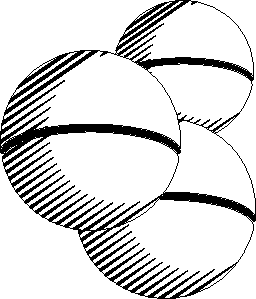
\includegraphics[width=0.21\textwidth]{frontispice-voix-des-airs.pdf}
	\caption{Ébauche de frontispice d’après l’œuvre de René \textsc{Magritte} \work{La Voix des airs}.}
	\vspace{-2.0em}
\end{wrapfigure}
\
\
{\em\normalsize Discours sur le frontispice.}~
Guerre de tous contre tous parce que cette Arche est en réalité un radeau certes, un radeau de la \emph{Méduse} de surcroit qui vogue dans l’espace pendant trente millénaires et dont il n’est aucun \emph{Argus}. Si alors \textsc{Géricault} aurait été bien indiqué pour tracer le frontispice de cet ouvrage, c’est en réalité Abraham \textsc{Bosse} qui prévalut, le graveur de celui du \work{Léviathan}\footcite{leviathan}. Car là dessus, il m’a semblé qu’une vision iconique et d’aucun jugerais même magritienne était fort à propos. Celle d’un échiquier céleste où les astres sont autant de pièces. Bien qu’à ce propos je nourrisse trois regrets. Le premier, étant qu’\elena{} qui figure le camp \enquote{égyptien} se serait plus judicieusement vu flanqué d’un plateau de senet mais alors l’image qu’en aurait eu un observateur contemporain aurait été moins explicite. Le deuxième, est que les Voyageur de l’Arche ne constituent pas, ou pas encore, une civilisation intergalactique mais se cantonnent à un seul véhicule spatial qui est leur seul lieu de vie. La troisième, étant que, pour paraphraser le grand maitre international M.\,Garry \textsc{Kasparov} \incise{quoiqu’il ai dit la chose au sujet de M.\,Vladimir \textsc{Putin}} \elena{} Skylab est davantage un joueur de poker, qui bluff, ne montre pas ses cartes et encore moins ses atouts. Ainsi, le jeu de la politique n’est pas, selon la classification établie par Jérôme \textsc{Cardan} et complétée par Godefroid-Guillaume \textsc{Leibniz}, un jeu à information complète et parfaite. L’on pourrait d’ailleurs s’interroger sur le fait que cette caractéristique, celle du degrés de  connaissance par l’ensemble des agents politiques des tenants et aboutissants d’une situation, serait  un bon discriminant qui distinguerait les régimes politiques saints des régimes déviants. La question demeurant ouverte, elle est un avis aux doctorants en manque d’inspiration pour leur sujet de thèse.

\begin{wrapfigure}{o}[3cm]{5.5cm}
	\vspace{-1em} % TODO ajustement en dur
	\centering
	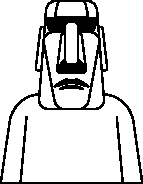
\includegraphics[width=0.2\textwidth]{frontispice-moai.pdf}
	\caption{Ébauche de frontispice représentant un moaï de l’île de Pacques. Statue dont la construction semble avoir été cause du déclin de la population de l’île.}
	%\vspace{-10pt}
	\vspace{-4em} % TODO ajustement en dur
\end{wrapfigure}
\
\
{\em\normalsize Finitude du lieux.}~
Quelque soit ce jeu, il est certain qu’il se joue sur un plateau dont les bords coïncident avec la coque de l’Arche. Car il faut bien un huit-clots à cette Arche rapanui, pour qu’ai  lieux  l’holocauste permanent étalé sur trente millénaires, et entretenu par une société assoiffée de ressources. Mais ce n’est pas une lutte pour les ressources vitales mue par la pression écologique et la pénurie. C’est une lutte pour l’accaparement des ressources de confort qui non seulement préfigure\footnote{Je devrais dire \autonym{postfigure} vue que les événements de l’intrigue sont sensés se dérouler dans des milliers d’années.} notre société de consommation actuelle, mais plus encore \incise{et aucun point de Godwin ne sera atteint} le nazisme qui nous est, bien plus que nous le croyons, proche.

\paragraph{Lutte pour le niveau de vie}
La lutte n’est pas vitale, car les principaux protagonistes de la haute société du Pont pas plus que les ouvriers de la Cale, ne pâtissent de  la faim et ne semblent guère plus menacés par la famine. En revanche, les aristocrates et tous ceux qui en ont le pouvoir sont mus par l’avidité pour les ressources de confort. Celles qui leur permettront d’attiser l’admiration en société, d’acquérir plus de pouvoir, de soutiens, de faire étalage de luxe, et si possible d’un luxe inutile. Ce que les économistes appelleraient aujourd’hui des bien positionnels ou des biens de consommation ostentatoires. Et ce, comme un \textsc{Hitler} se lancerait à la poursuite d’un \xenism{lebensraum} ou \enquote{espace vital} mu par une panique écologique comme dirait M.\,Timothy \textsc{Snyder}\footcite{timothySnyder2016Gallimard-TerreNoire}. Car il m’a semblé que la folie meurtrière d’\textsc{Hitler} ne se suffit pas du seul suprémacisme pour explication, mais à ce suprémacisme  doit s’adjoindre le second facteur qu’est la recherche à mort de nutriments, de ressources, de biens, de services si possible accomplis par une main d’œuvre servile. Et ce, \incise{non pas afin de se contenter de survivre}, non car voilà une prétention tout juste bonne pour les sots, mais en revanche pour acquérir le plus haut niveau de vie possible, voir une prospérité sardanapalesque.

%Finalement, la pression écologique n’est pas due à la surpopulation mais à la surconsommation de quelques uns qui refusent obstinément qui refusent obstinément aux autres d’accéder aux ressources.

\paragraph{Modernité de la lutte}
{\em\normalsize Chez les aristocrates.}~
Si donc dans le monde intérieur de l’Arche, il ne semble pas y’avoir de crise écologique comme dans le notre qui est bien réel, eh bien qu’importe ai-je envie de dire. Car quelque soient les ressources à disposition, les puissants auront toujours tout autant envie de s’en accaparer le plus possible, au delà du nécessaire, au détriment des autres, quitte à engendrer une pénurie organisée. \autonym{Quitte}, ai-je dis ? Que je loue mon attendrissante naïveté ! C’est \autonym{pour} engendrer une pénurie organisée, car plus misérables sont les gueux et plus magnifiques seront les puissants.
Ce n’est pas une lutte pour la survie, c’est une lutte pour le confort et le niveau de vie. %Comme dans l’incipit d’Herbert George \texts{Wells} où le Anglais génocident toute la population de Nouvelle-Zéllande afin que \enquote{les moutons anglais puissent continuer de paitre}.
C’est le cynisme amené à son terme, où pour ne pas se gêner dans sa jolie et doucereuse promenade matinale, pourquoi hésiter à exterminer tous ceux qui croiseraient notre chemin, eux dont les vieux haillons troués jurent avec l’allée de cyprès taillés ? Oh, et puis maintenant que l’idée est évoquée, autant les exterminer préventivement, dites ! La promenade n’en sera que plus agréable et cela donnera le temps aux équipes de salubrité publique de recycler les dépouilles afin d’en faire un engrais bon à accroitre le rendement des fleures d’apparat qui jalonneront notre encore plus belle promenade. Et dans cette ingénierie du mal, l’on se surprendra même à être admiratif devant notre brillante idée, étalant un sourire carnassier d’autosatisfaction.

Et le propos n’est pas du tout exagéré. \textsc{Hitler} disait qu’à l’édification du \enquote{jardin d’Éden germanique \textelp{} la meilleure manière d’atteindre ce résultat est d’abattre quiconque ose nous regarder de travers}%
\footcite[La citation est tirée des notes de \textsc{Bormann}, présentées en tant que preuve lors du procès de Nuremberg.][]{chirstopherBrowning2022BellesLettres-politiqueNazieTravailleursJuifsBourreauxAllemands}%
.

Il n’est donc pas simplement question de vie, mais de niveau de vie. D’aucun dirait de \xenism{layfe stayle}, sous l’égide du néolibéralisme triomphant avec son cortège de développement personnel et d’idéologie managériale, psalmodiée par ses armées d’influenceurs.

C’est donc une lutte, le répète M.\,Timothy \textsc{Snyder}, pour le confort.  La quête d’Hitler pour le \xenism{lebensraum} est une quête, non pas archaïque comme on se le figure, non pas pour de basses et terre-à-terre considérations de survie, mais une quête bien plus proche qu’on ne le souhaiterait de nos sociétés de consommation modernes. S’il est vrais qu’à la suite des accords de Versailles on meure \incise{au sens propre} de faim en Allemagne et que les dirigeants et théoriciens nazis connurent la faim, Hitler écrit néanmoins \enquote{Il est normal de nous \textins{les Allemands} sentir anxieux car nous devons posséder toujours plus, encore plus.}.

Aussi, la haute société de la cour archienne, quoique parée de toutes les commodités utiles et même superflues, semble malgré tout baigner dans une espèce de menace de précarité. Car sont mobilisés des imaginaires liés au dénuement à l’état primitif, aux menaces de la nature, celle de la prédation, de la faim, et des aléas de l’existence animale.
C’est que la rhétorique que déploie cet imaginaire suscite des émotions prétendument survivalistes, à l’appuis de ce qui est en réalité une guerre pour un niveau de vie.

{\em\normalsize Chez les ouvriers.}~
À l’autre bout du spectre, chez les ouvriers de la Cale, cette logique est similaire à la mort lente dans les camps appelées \enquote{Réduction naturelle} par administration de moins de nutriment qu’il n’en faut à la survie des prisonniers comme en témoigne le rapport de la conférence de Wannsee du 1940 janvier 20. Mais à la différence des nazis, l’Intelligentsia de l’Arche a poussé le vice au point que les ouvriers soient génétiquement conçus pour décéder (le texte dit \enquote{tomber en fin de service}, participant de leur déshumanisation) tout juste à soixante-quatre ans lorsqu’ils atteignent l’âge de la retraite. Soit une optimisation de la charge non pas seulement salariale mais même sociale que représente un ouvrier, que ne nierait pas le \xenism{New Public Management}. Oh tiens, ai-je parlé de \xenism{New Public Management} ?
Ne serait-ce pas le nouveau nom dégérmanisé de la \xenism{menschenführung} apportée aux ÉUA par les transfuges nazis ? Cette science qui cherche à tirer le meilleur profit du minerai d’humain  et que l’on a anglicisé au sortir de la guerre pour la parer d’une respectabilité dont la privait la consonance allemande encore trop suspecte à l’époque ?
\footcite{JohannChapoutot-NRF2020-libresDObéir}


%Si donc, l’ascenssion d’\elena{} Skylab, traite comme son nom l’indique de ce vol de l’aigle du personnage éponyme et n’est pas un univers étendu à la façon de Dune ou Star Trek, et que n’y sont pas traités la genèse de l’arche, les condition historiques et politique du Jactum de l’Arche, ni même les différentes époques intérmédiaires des trentes millénaires de l’hisotire de l’arche, 
%L’on pourrait alors présager que le 

\paragraph{\elena{} dans la tourmente}
\begin{wrapfigure}{o}[3cm]{5.5cm}
	\vspace{-1em}
	\centering
	
\includegraphics[width=0.2\textwidth]{frontispice-arche-evidee.pdf}
	\caption{Ébauche de frontispice représentant une forme hypothétique d’un vaisseau transgénérationnel ayant la forme d’un anneau.}
	\vspace{-10pt}
\end{wrapfigure}
\
\
{\em\normalsize Le savoir comme clé de voute.}~
Ainsi posées les structures sociales, ou plus exactement les \emph{infrastructures}, contraignantes ne laissant de place qu’à la violence de ceux ayant les moyens de la déployer, \elena{} cherche à tirer son épingle du jeu.
Et il n’y est fait que peu de place à l’erreur. Et sans doute est-ce du à son ambivalence, quoiqu’atténuée par son affiliation à la faction égyptienne, qu’\elena{}  doit son salut, tout du mois sa singularité.

À commencer par son état-civil qui fait montre d’un prénom grec, quoique l’on pourrait l’imaginer héléno-égyptien ainsi que semble le suggérer le nom dont il baptise sa fille homonyme (ou éponyme ?) de la dernière des Lagides. Et ce alors que son nom de famille est germanique. Mais à vrais dire, qu’importe, car ce pourquoi il réussi n’est pas dû à ce qu’il est lui, son égyptianité n’ayant pratiquement jamais part, mais à ce que sont les autres et à la virtuosité par laquelle il s’articule avec. S’il réussi, c’est parcequ’il semble avoir mieux lu Sun~Tzu que \reine, mieux appliqué les techniques de renseignement des Viking que \princesse, et mieux écouté les enseignements de la métis d’Ulysse que \general. Lui qui n’a pas mangé leur chaires a mangé leur connaissances. N’ayant ni leur prébende ni leur pouvoirs, c’est son savoir qui lui en confèrera un. Ou plus exactement le savoir de ses ennemis dont il s’est accaparé. Ah quelle éloquente homophonie entre \emph{savoir} et \emph{pouvoir} que nous offre là la langue française. Que je plein d’amblais les traducteurs germanophones qui auront le déplaisir d’écrire \xenism{wissen} et \xenism{leistung}, ou les arabophones pour \xenism{ma\fallbackserif{ȝ}rifaẗ} et \xenism{sultaẗ}, et sinophones pour \xenism{zhīdào} et \xenism{lìliàng}.
Aussi sommes-nous tentés de railler \general{} au delà de la mort, lui qui ne manqua pas d’initier la métaphore du papier des grimoires qui est le linceul des savants, car en filant sa propre métaphore, enroulé, ce papier-là devient sceptre. Oh, et tant qu’à être d’humeur lyrique et imagée, faisons lui remarquer que son bâton de maréchal n’est plus que la rame qui lui servira de canoter sur l’Avalon, car mort dans l’indignité ce Grec n’aura pas de drachme dans sa bouche pour payer Charon. % Vérifier le nom de Chauron
Puisqu’enfin le {savoir} dont il est question ici, à l’instar de l’anthropophagie, confondra le sens figuré au sens propre. C’est le savoir du maitre espion qui n’agit que fort précautionneusement, et c’esst le savoir du scientifique qui ne délibère qu’avec prudence, autant dire alors la sagesse.

{\em\normalsize Cynisme d’\elena{}.}~
%> Mais \elena{} n’est certainement pas un humaniste idéaliste
Toute fois, et parce que voguant dans l’océan de mépris et de cruauté, \elena{} Skylab en homme de son temps, n’est pas moins intraitable que les autres. Si le tranchant de son épée rate son adversaire, il ne manquera pas de l’assommer avec le pommeau de la poignée. Manquerait-il de flèches à encocher à son arc que le carquois vide lui servira de gourdin. Et pourtant, à aucun moment le long de la pièce il ne tiendra de sa propre main une arme. Il ne mandate pas même des assassins à sa solde pour exécuter ses basses besognes. Il fait en sorte que ses ennemis aient l’air de se saboter d’eux mêmes, ou mieux se sabotent entre eux. Ça fera des économies, tiens. Lors son savoir opère.

Un juge d’instruction libre et ayant tous les moyens d’enquêter sur la responsabilité d’\elena{} aurait beaucoup de mal à l’inculper, tant ses manigances sont sinueuses. L’accuserait-on d’avoir assassiné \princesse ? Mais enfin, elle s’acharna d’elle même à vouloir partir à la guerre où elle a été tuée par les ennemis ; et puis à la guerre on meure, ça ne s’invente pas. Ces ennemis là bénéficièrent-ils d’une trahison ? C’est évidement \vladimir{} qui en est l’auteur vue qu’il a reçu la solde de sa délation ; et ça tombait bien il manquait d’argent. Compte à \general, il est mort de sa propre ambition. Et enfin, \roi{} n’a-t-il pas de lui même saisi en connaissance de cause la fiole de cigüe pour se suicider ? Notre pauvre et persécuté orphelin \elena{} n’est qu’une victime au milieu du tumulte. Quel esprit malfaisant oserait l’accuser ? Qui l’oserait ?

Finalement, le regret que je nourris est celui qu’\elena{} n’ai pas lui même, ni à travers son entourage, eut à déplorer de perte. La tragédie semble toucher les autres. Je regrette sans doute qu’\elena{} ai trop bien joué son rôle. Voilà le défaut que je me reproche. Ce n’est certes pas un Gary-Stu, car il est ce que les anthropologues noment en termes scientifiques un \autonym{connard}, mais c’est tout du moins un Gary-Sue intellectuel.


\paragraph{Structure et thématiques}
\begin{figure}[!t]
  \marginnote{\null\vspace{0.68cm}\\ \footnotesize\fullcite{FNP-drame}.}
	\centering
	\includegraphics[width=\textwidth]{drame.pdf}
	\caption{Planche de blog bd réalisées lors de l’achèvement de cette pièce, quoique le ressors comique mis en œuvre relève d’un humour compréhensible des programmeurs.}
\end{figure}
Le  propos abordé par cette pièce est certes éminemment celui de notre siècle qui a, non pas vingt-trois ans, mais cent-neuf. Car il s’agit toujours du même siècle commencé dans une rue de Sarajevo et qui ne prit toujours pas fin en 1991, n’en déplaise à M.\,Francis \textsc{Fukuyama}. Toute fois, la structure compte à elle emprunte au théâtre classique français avec ses obstinés cinq actes parce que j’ai été dressé par l’école française à suivre ce modèle autant racinien que cornélien. Dressage dont j’ai toute fois grignoté la laisse en manquant allègrement aux unités de lieu, d’intrigue, et de temps, ainsi qu’à l’observance de la bienséance. Et je dois avouer que cette transgression fut d’une exquise salvation. Ma maitresse de français qu’enfant je voyais avec les yeux qu’un \textsc{Rousseau} avait pour Thérèse \textsc{Levasseur}, devint dans les moments où j’enfreignais toutes ces règles une Merteuil qui cède aux asseaux de Valmont. Toute fois, si la structure tient au théâtre classique français, l’intrigue et les relations interpersonnelles empruntent au théâtre élisabéthain. Le roi Agamemnon qui devient fou est probablement une incarnation de Lear tandis que les formules aussi stéréotypées qu’énigmatiques où les prémonitions parsemées ici et là tiennent quelque chose des sorcières de \work{Macbeth}.

Car il m’a semblé qu’entre deux merlons l’un cachant Christophe \textsc{Marlowe} et l’autre Pierre \textsc{Corneille}, il devait y’avoir un créneau, celui depuis lequel nous apparait Bertolt \textsc{Brecht}.

%chav, racaille, rude boys, gopnik, bouzabbal, douchebag, zef
